

%%%%
%%%%  FIGURE
%%%%
%\begin{landscape}
\begin{figure}[ht] 
\vbox{\vspace{-1cm}
\centering
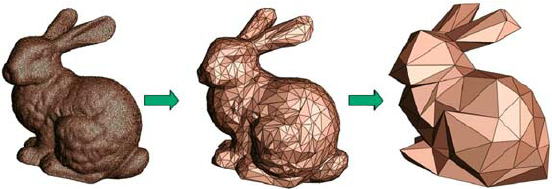
\includegraphics[width=.56\textwidth]{./Pics/Introduction/Graphical-illustration-of-model-order-reduction.png}
\vspace{0.cm}
\vspace{0.5cm}
}   
\caption{Graphical illustration of model order reduction (initially used by \citet{Schilders2008}, with graphics credited to Harvard University, Microsoft Research.)}
\vspace{1.5cm}
\label{fig:IllustrationMOR}
\end{figure}

\begin{figure}[ht] 
\vbox{\vspace{-1cm}
\hbox{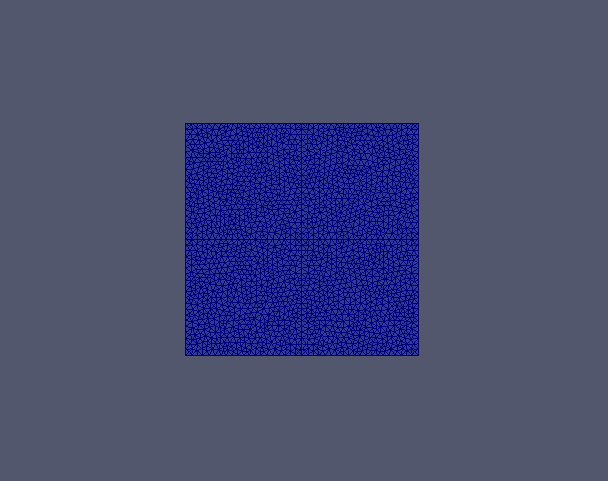
\includegraphics[width=.56\textwidth]{./Pics/BaseCase/BaseCase_MeshOnly.png}
      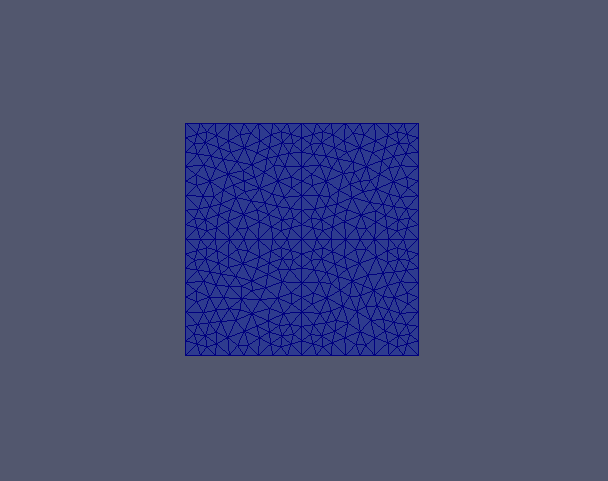
\includegraphics[width=.56\textwidth]{./Pics/ArithMeanCase/ArithMeanCase_MeshOnly.png}}
\vspace{0.cm}
\hbox{\hspace{0.25cm} (a) High Resolution Grid (BaseCase) \hspace{0.75cm} (b) Low Resolution Grid (Upscaled Cases) \hspace{3.0cm}}
\vspace{0.5cm}
}   
\caption{Simulation grid for the high resolution case and the upscaled cases}
\label{fig:HiRes_LowRes_Mesh}
\end{figure}


%\end{landscape}
\clearpage



%%%%
%%%%  FIGURE
%%%%
\begin{landscape}
\begin{figure}[ht] 
\vbox{\vspace{-1cm}
\hbox{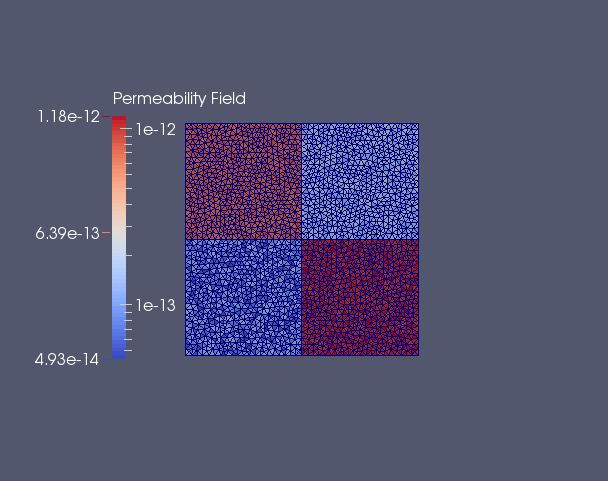
\includegraphics[width=.56\textwidth]{./Pics/BaseCase/BaseCase_PermField_withMesh.png}
      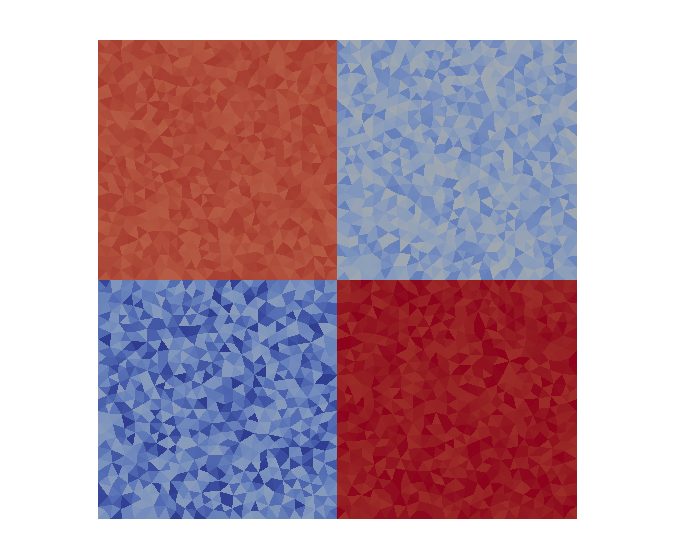
\includegraphics[width=.56\textwidth]{./Pics/BaseCase/BaseCase_PermField_withoutMesh2.png}
      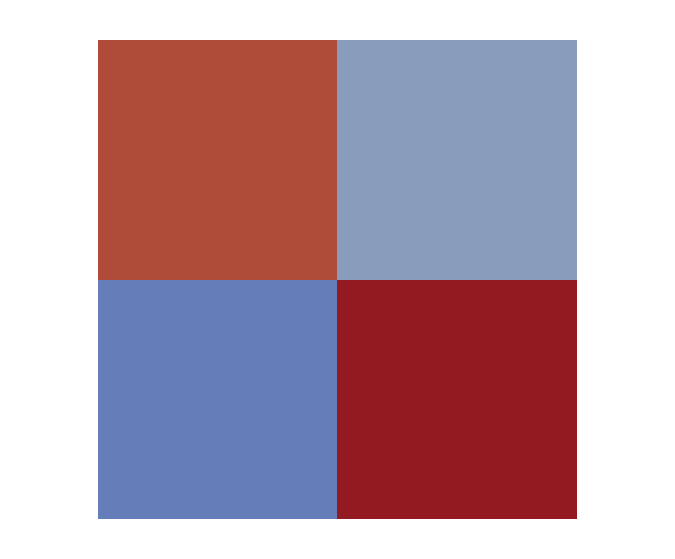
\includegraphics[width=.56\textwidth]{./Pics/ArithMeanCase/ArithMeanCase_PermField_withoutMesh2.png}}
\vspace{0.cm}
\hbox{\hspace{0.5cm} (a) BaseCase(with mesh) \hspace{3.75cm} (b) BaseCase(without Mesh) \hspace{3.0cm} (c) ArithMean Case}
\vspace{0.5cm}
\hbox{
      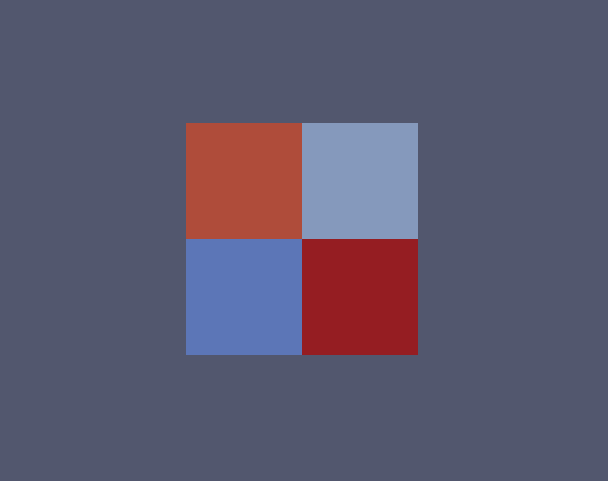
\includegraphics[width=.56\textwidth]{./Pics/HarmMeanCase/HarmMeanCase_PermField_withoutMesh2.png}
      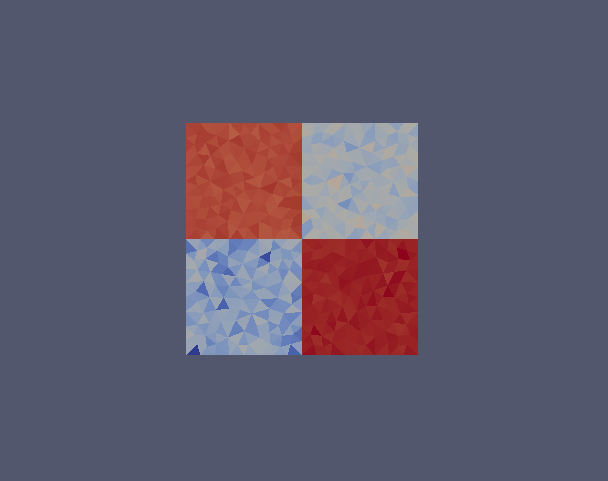
\includegraphics[width=.56\textwidth]{./Pics/PDFCase/PDFCase_PermField_withoutMesh2.png} 
      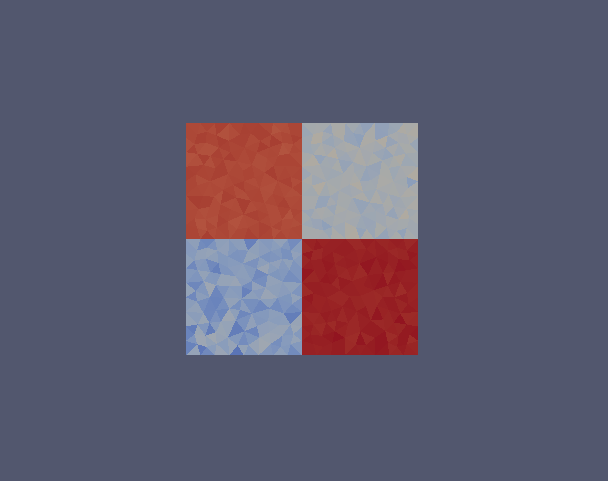
\includegraphics[width=.56\textwidth]{./Pics/SVDCase/SVDCase_PermField_withoutMesh2.png}}
\vspace{0.cm}
\hbox{ \hspace{1.5cm} (d) HarmMean Case \hspace{4.75cm} (e) PDFCase  \hspace{5.0cm} (f) SVDCase}
\vspace{0.cm}
}   
\caption{Permeability field for the base case as well as the upscaled cases}
\label{fig:PermFields}
\end{figure}
\end{landscape}
\clearpage


%%%%
%%%%  FIGURE
%%%%
\begin{landscape}
\begin{figure}[ht] 
\vbox{\vspace{-1cm}
\hbox{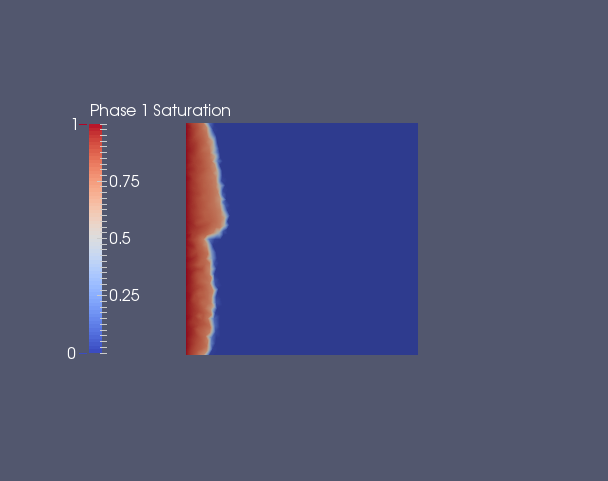
\includegraphics[width=.56\textwidth]{./Pics/BaseCase/BaseCase_Saturation_t_dot15.png}
      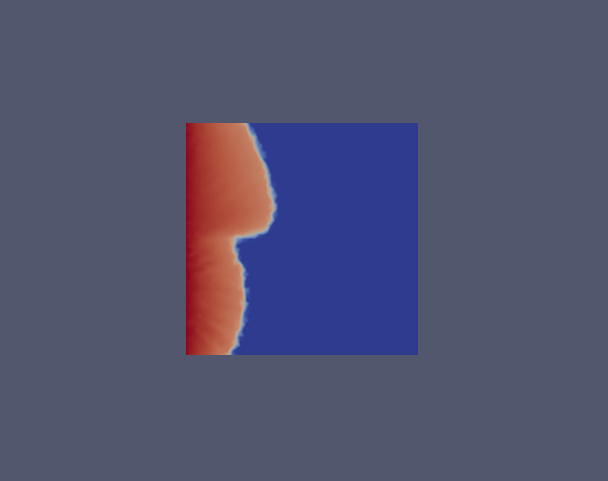
\includegraphics[width=.56\textwidth]{./Pics/BaseCase/BaseCase_Saturation_t_dot30.png}
      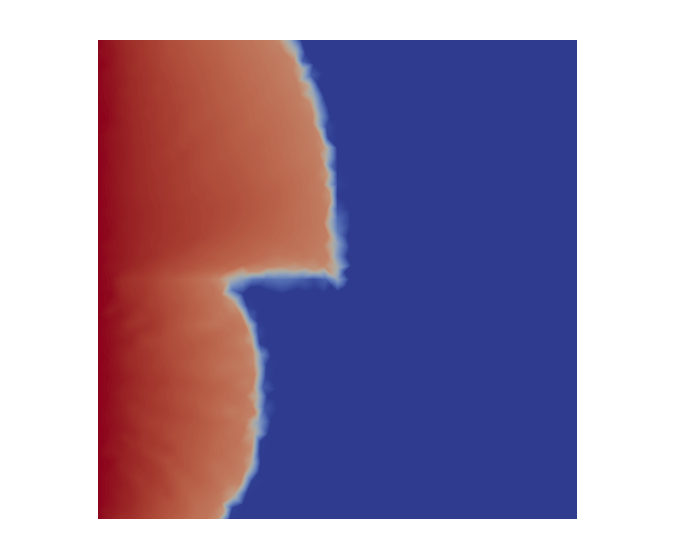
\includegraphics[width=.56\textwidth]{./Pics/BaseCase/BaseCase_Saturation_t_dot50.png}}
\vspace{0.cm}
\hbox{\hspace{0.5cm} (a) Phase 1 Saturation at t=0.15s \hspace{3.75cm} (b) t=0.30s \hspace{5.0cm} (c) t=0.50s}
\vspace{0.5cm}
\hbox{
      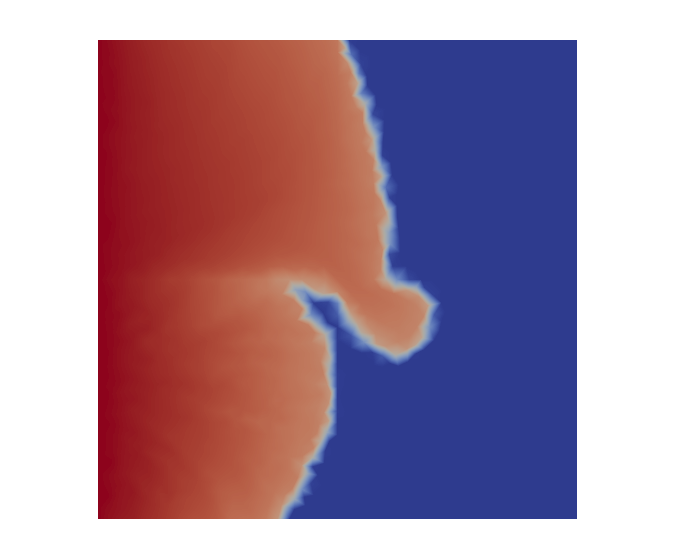
\includegraphics[width=.56\textwidth]{./Pics/BaseCase/BaseCase_Saturation_t_1dot15.png}
      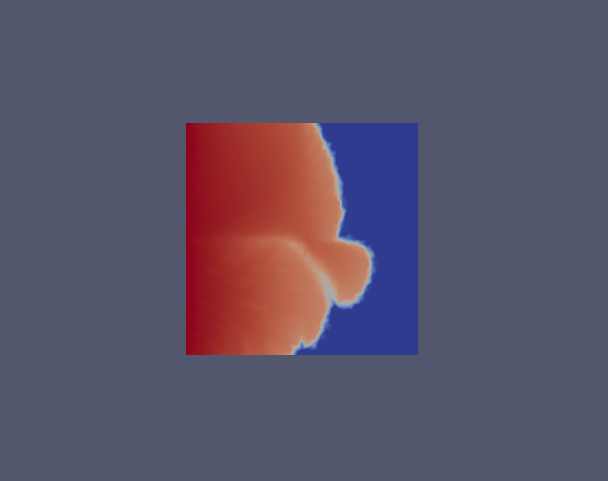
\includegraphics[width=.56\textwidth]{./Pics/BaseCase/BaseCase_Saturation_t_1dot75.png} 
      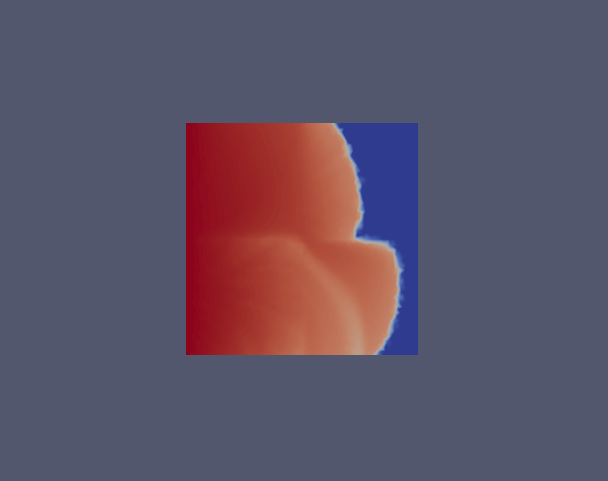
\includegraphics[width=.56\textwidth]{./Pics/BaseCase/BaseCase_Saturation_t_2dot95.png}}
\vspace{0.cm}
\hbox{ \hspace{2.5cm} (d) t=1.15s \hspace{5.5cm} (e) t=1.75s   \hspace{5.5cm} (f) t=2.95s}
\vspace{0.cm}
}   
\caption{Simulations for the BaseCase}
\label{fig:BaseCase_Saturation}
\end{figure}
\end{landscape}
\clearpage


%%%%
%%%%  FIGURE
%%%%
\begin{landscape}
\begin{figure}[ht] 
\vbox{\vspace{-1cm}
\hbox{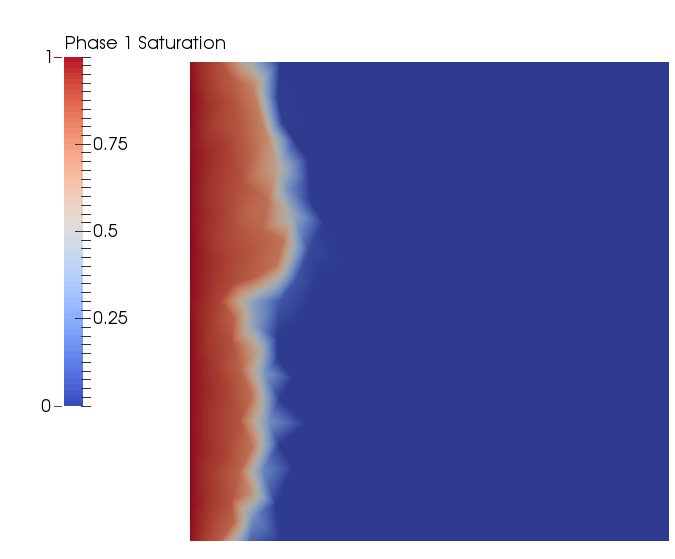
\includegraphics[width=.56\textwidth]{./Pics/ArithMeanCase/ArithMeanCase_Saturation_t_dot15.png}
      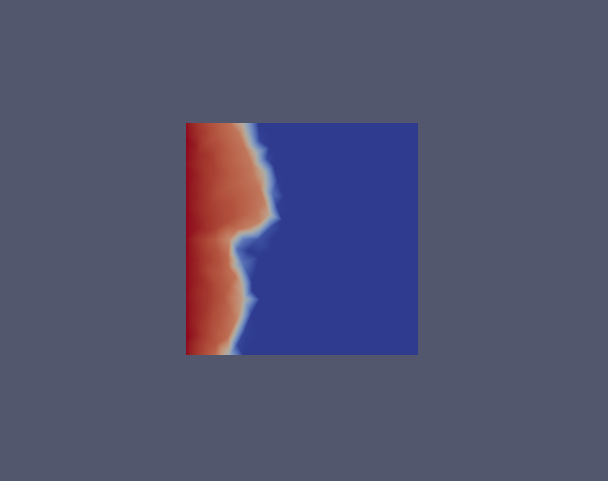
\includegraphics[width=.56\textwidth]{./Pics/ArithMeanCase/ArithMeanCase_Saturation_t_dot30.png}
      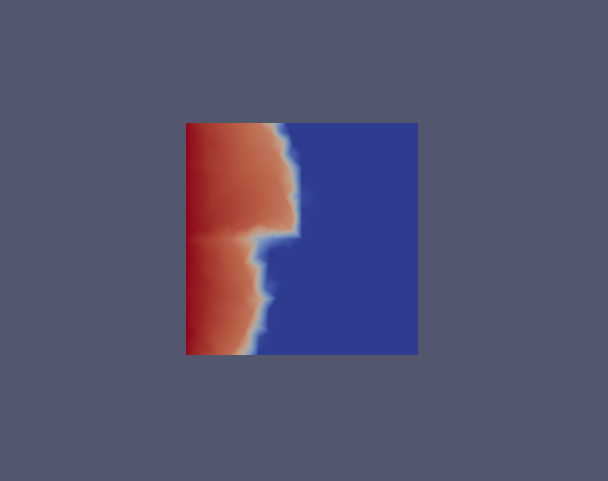
\includegraphics[width=.56\textwidth]{./Pics/ArithMeanCase/ArithMeanCase_Saturation_t_dot50.png}}
\vspace{0.cm}
\hbox{\hspace{0.5cm} (a) Phase 1 Saturation at t=0.15s \hspace{3.75cm} (b) t=0.30s \hspace{5.0cm} (c) t=0.50s}
\vspace{0.5cm}
\hbox{
      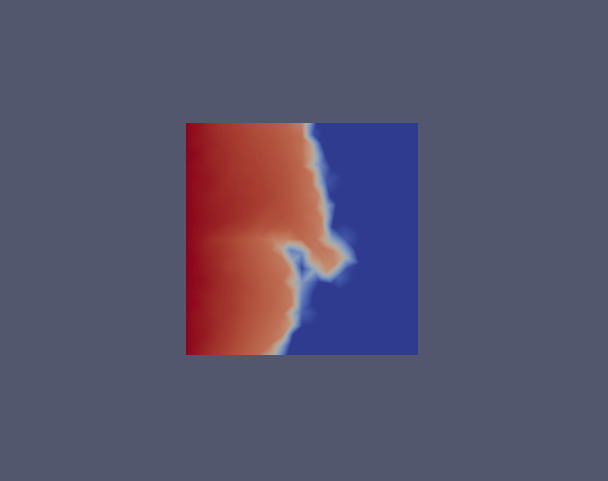
\includegraphics[width=.56\textwidth]{./Pics/ArithMeanCase/ArithMeanCase_Saturation_t_1dot15.png}
      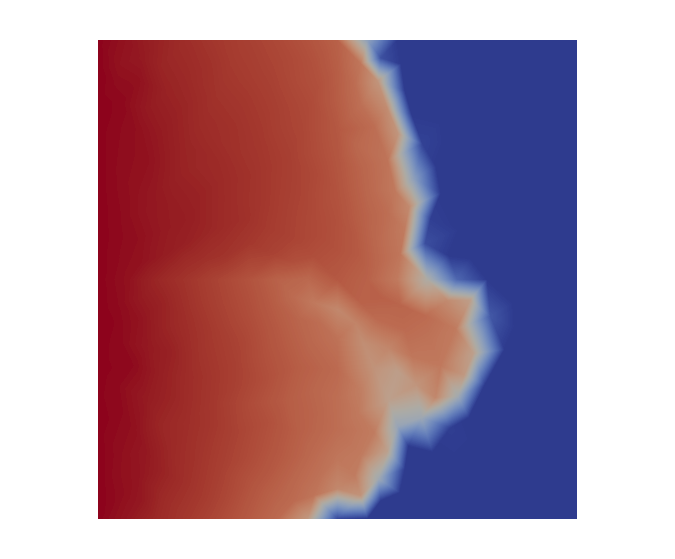
\includegraphics[width=.56\textwidth]{./Pics/ArithMeanCase/ArithMeanCase_Saturation_t_1dot75.png} 
      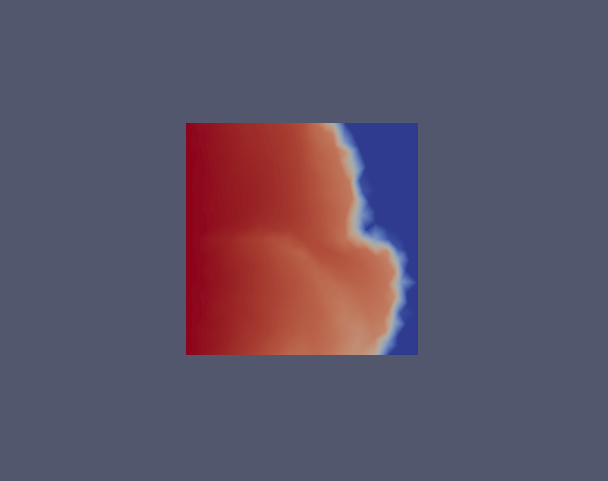
\includegraphics[width=.56\textwidth]{./Pics/ArithMeanCase/ArithMeanCase_Saturation_t_2dot95.png}}
\vspace{0.cm}
\hbox{ \hspace{2.5cm} (d) t=1.15s \hspace{5.5cm} (e) t=1.75s   \hspace{5.5cm} (f) t=2.95s}
\vspace{0.cm}
}   
\caption{Simulations for the ArithMean Case}
\label{fig:ArithMeanCase_Saturation}
\end{figure}
\end{landscape}
\clearpage



%%%%
%%%%  FIGURE
%%%%
\begin{landscape}
\begin{figure}[ht] 
\vbox{\vspace{-1cm}
\hbox{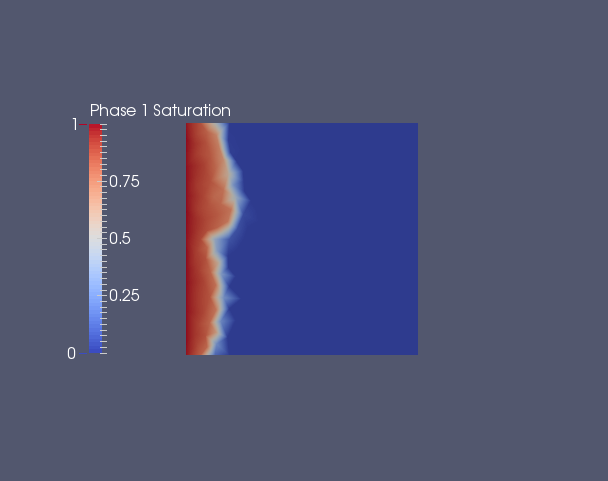
\includegraphics[width=.56\textwidth]{./Pics/HarmMeanCase/HarmMeanCase_Saturation_t_dot15.png}
      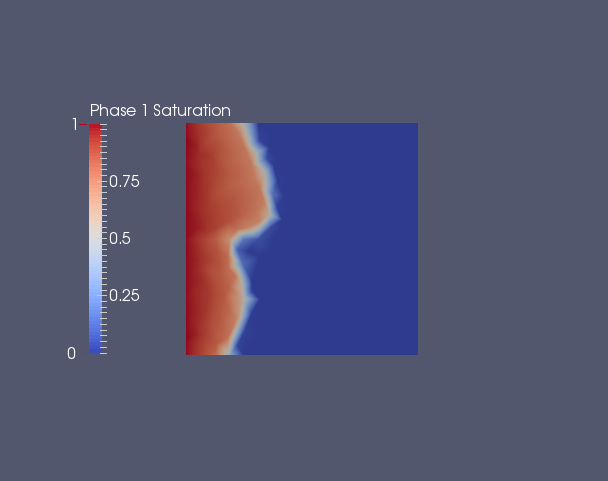
\includegraphics[width=.56\textwidth]{./Pics/HarmMeanCase/HarmMeanCase_Saturation_t_dot30.png}
      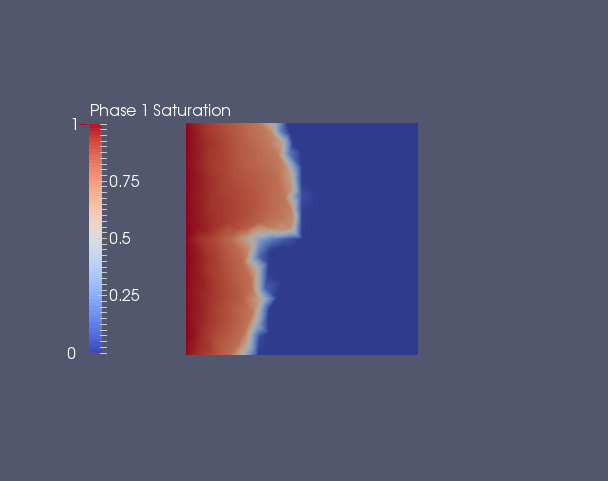
\includegraphics[width=.56\textwidth]{./Pics/HarmMeanCase/HarmMeanCase_Saturation_t_dot50.png}}
\vspace{0.cm}
\hbox{\hspace{0.5cm} (a) Phase 1 Saturation at t=0.15s \hspace{3.75cm} (b) t=0.30s \hspace{5.0cm} (c) t=0.50s}
\vspace{0.5cm}
\hbox{
      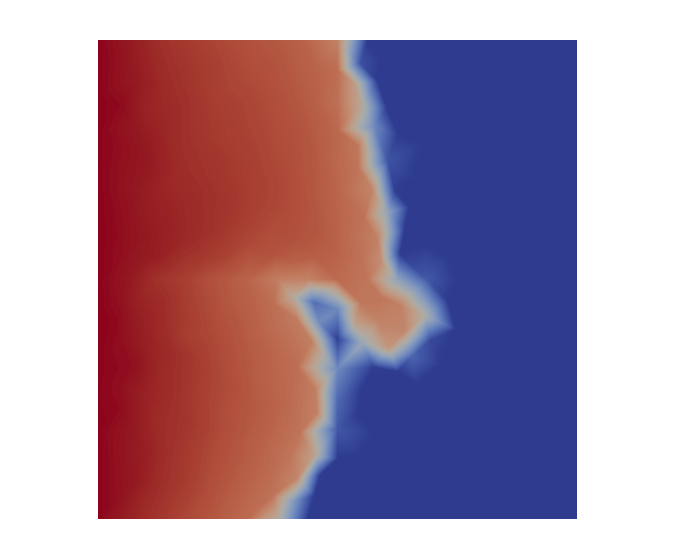
\includegraphics[width=.56\textwidth]{./Pics/HarmMeanCase/HarmMeanCase_Saturation_t_1dot15.png}
      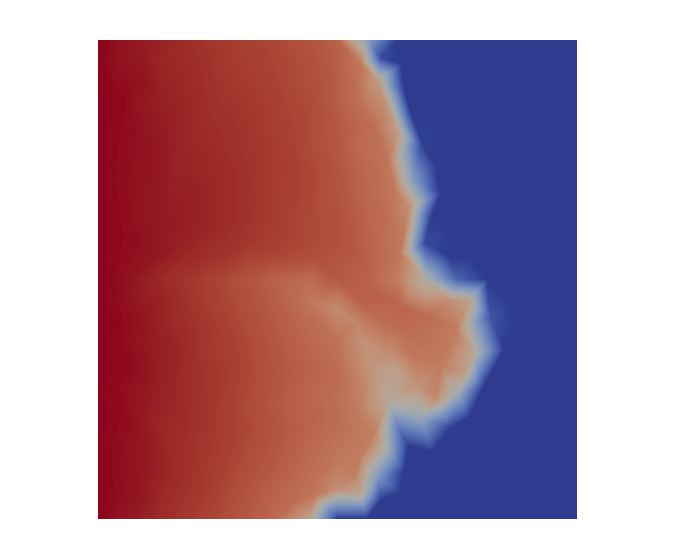
\includegraphics[width=.56\textwidth]{./Pics/HarmMeanCase/HarmMeanCase_Saturation_t_1dot75.png} 
      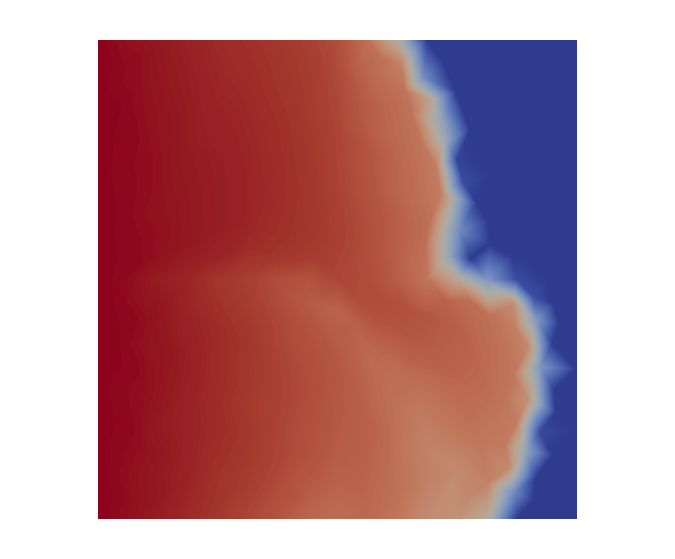
\includegraphics[width=.56\textwidth]{./Pics/HarmMeanCase/HarmMeanCase_Saturation_t_2dot95.png}}
\vspace{0.cm}
\hbox{ \hspace{2.5cm} (d) t=1.15s \hspace{5.5cm} (e) t=1.75s   \hspace{5.5cm} (f) t=2.95s}
\vspace{0.cm}
}   
\caption{Simulations for the HarmMean Case}
\label{fig:HarmMeanCase_Saturation}
\end{figure}
\end{landscape}
\clearpage





%%%%
%%%%  FIGURE
%%%%
\begin{landscape}
\begin{figure}[ht] 
\vbox{\vspace{-1cm}
\hbox{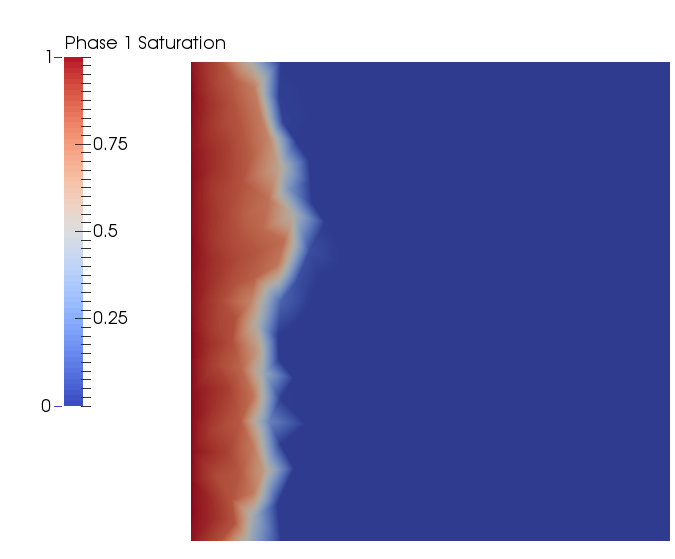
\includegraphics[width=.56\textwidth]{./Pics/PDFCase/PDFCase_Saturation_t_dot15.png}
      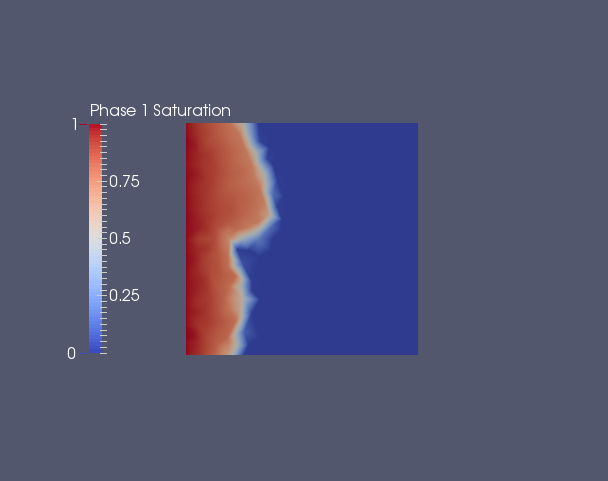
\includegraphics[width=.56\textwidth]{./Pics/PDFCase/PDFCase_Saturation_t_dot30.png}
      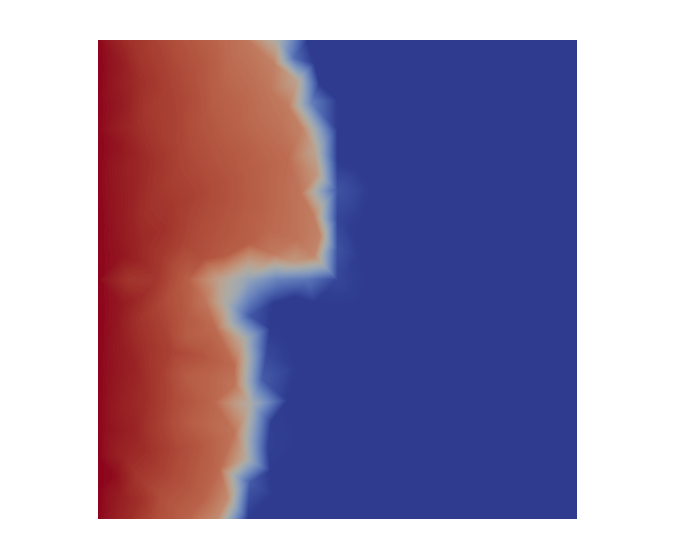
\includegraphics[width=.56\textwidth]{./Pics/PDFCase/PDFCase_Saturation_t_dot50.png}}
\vspace{0.cm}
\hbox{\hspace{0.5cm} (a) Phase 1 Saturation at t=0.15s \hspace{3.75cm} (b) t=0.30s \hspace{5.0cm} (c) t=0.50s}
\vspace{0.5cm}
\hbox{
      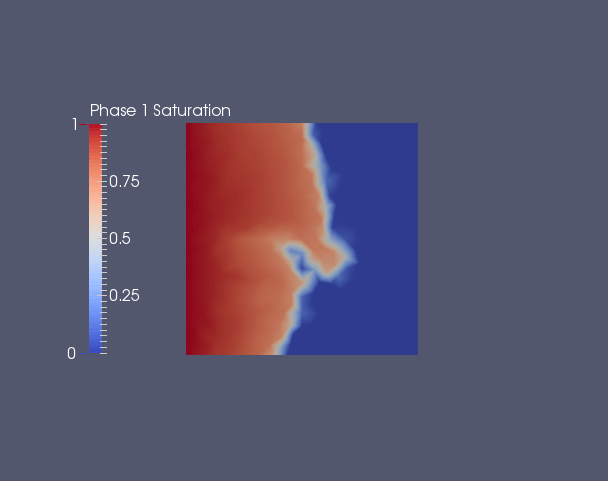
\includegraphics[width=.56\textwidth]{./Pics/PDFCase/PDFCase_Saturation_t_1dot15.png}
      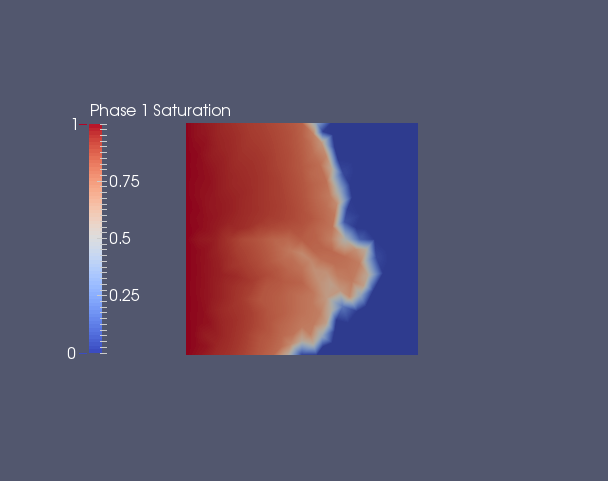
\includegraphics[width=.56\textwidth]{./Pics/PDFCase/PDFCase_Saturation_t_1dot75.png} 
      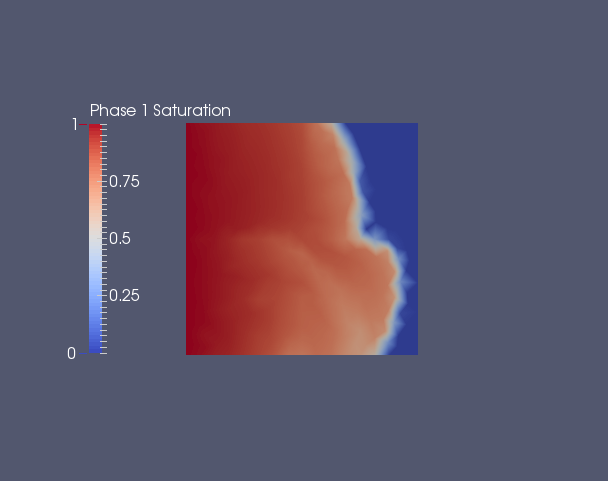
\includegraphics[width=.56\textwidth]{./Pics/PDFCase/PDFCase_Saturation_t_2dot95.png}}
\vspace{0.cm}
\hbox{ \hspace{2.5cm} (d) t=1.15s \hspace{5.5cm} (e) t=1.75s   \hspace{5.5cm} (f) t=2.95s}
\vspace{0.cm}
}   
\caption{Simulations for the PDFCase}
\label{fig:PDFCase_Saturation}
\end{figure}
\end{landscape}
\clearpage



%%%%
%%%%  FIGURE
%%%%
\begin{landscape}
\begin{figure}[ht] 
\vbox{\vspace{-1cm}
\hbox{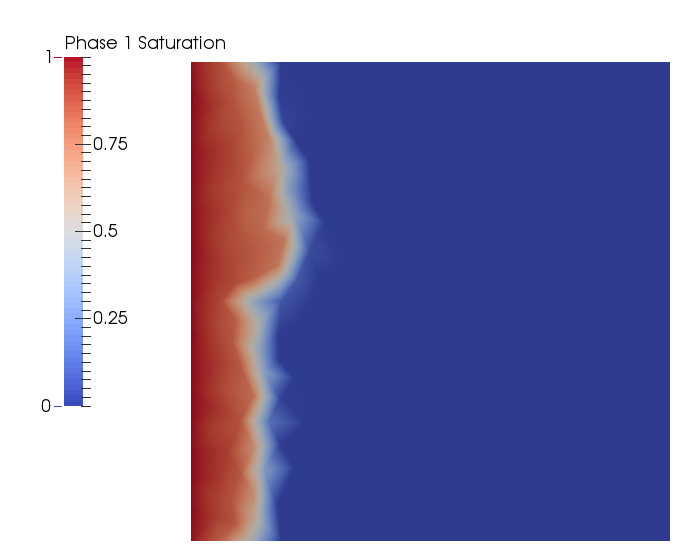
\includegraphics[width=.56\textwidth]{./Pics/SVDCase/SVDCase_Saturation_t_dot15.png}
      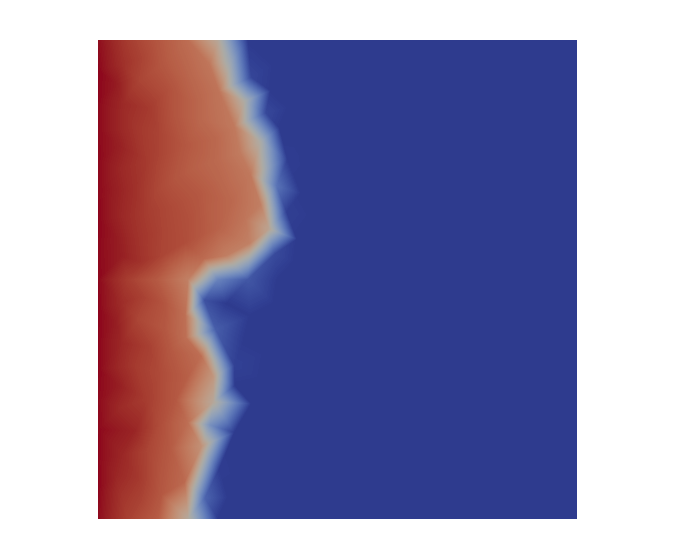
\includegraphics[width=.56\textwidth]{./Pics/SVDCase/SVDCase_Saturation_t_dot30.png}
      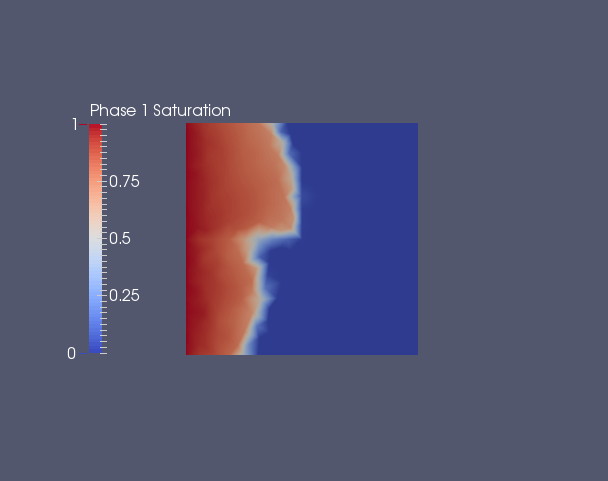
\includegraphics[width=.56\textwidth]{./Pics/SVDCase/SVDCase_Saturation_t_dot50.png}}
\vspace{0.cm}
\hbox{\hspace{0.5cm} (a) Phase 1 Saturation at t=0.15s \hspace{3.75cm} (b) t=0.30s \hspace{5.0cm} (c) t=0.50s}
\vspace{0.5cm}
\hbox{
      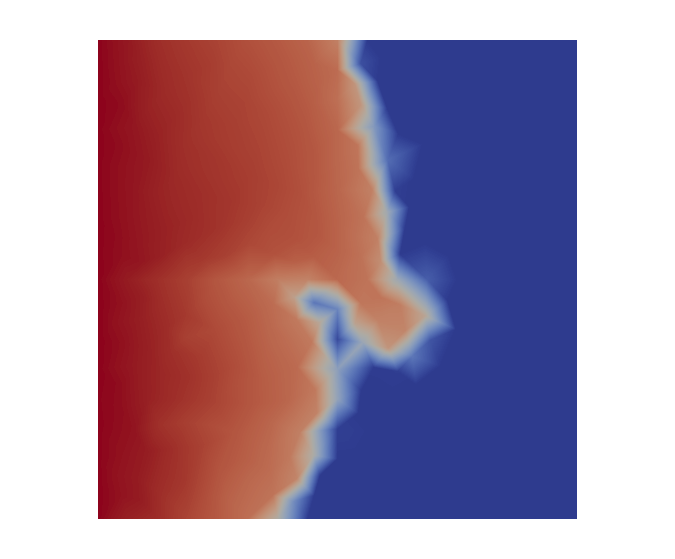
\includegraphics[width=.56\textwidth]{./Pics/SVDCase/SVDCase_Saturation_t_1dot15.png}
      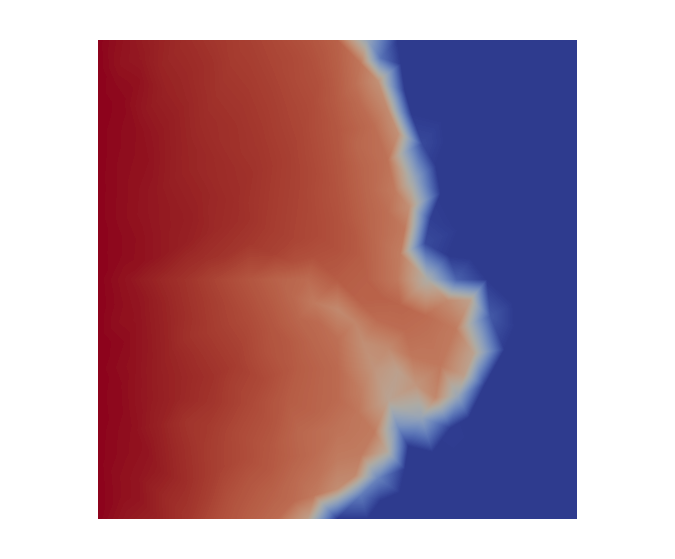
\includegraphics[width=.56\textwidth]{./Pics/SVDCase/SVDCase_Saturation_t_1dot75.png} 
      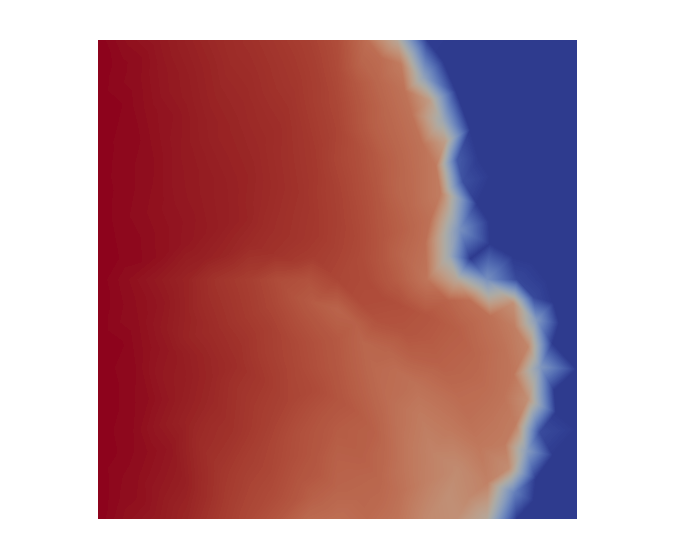
\includegraphics[width=.56\textwidth]{./Pics/SVDCase/SVDCase_Saturation_t_2dot95.png}}
\vspace{0.cm}
\hbox{ \hspace{2.5cm} (d) t=1.15s \hspace{5.5cm} (e) t=1.75s   \hspace{5.5cm} (f) t=2.95s}
\vspace{0.cm}
}   
\caption{Simulation for the SVDCase}
\label{fig:SVDCase_Saturation}
\end{figure}
\end{landscape}
\clearpage



%%%%
%%%%  FIGURE
%%%%
\begin{landscape}
\begin{figure}[ht] 
\vbox{\vspace{-1cm}
\hbox{\hspace{4cm} 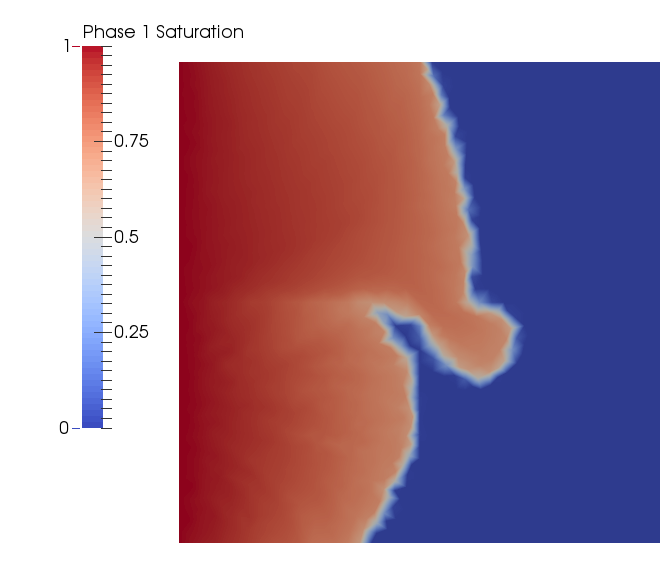
\includegraphics[width=.56\textwidth]{./Pics/BaseCase/BaseCase_Saturation_t_1dot15withlegend.png}
      \hspace {1.5cm} 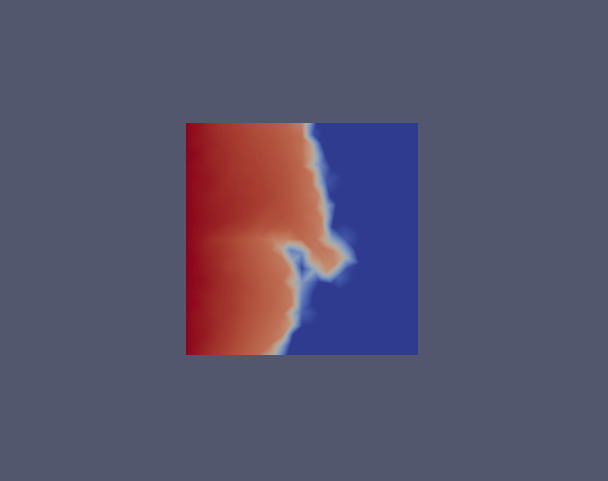
\includegraphics[width=.56\textwidth]{./Pics/ArithMeanCase/ArithMeanCase_Saturation_t_1dot15.png}}
\vspace{0.cm}
\hbox{\hspace{3.75cm} (a) BaseCase: Phase 1 Saturation at t=1.15s \hspace{1cm} (b) ArithMeanCase: Phase 1 Saturation at t=1.15s}
\vspace{0.5cm}
\hbox{
      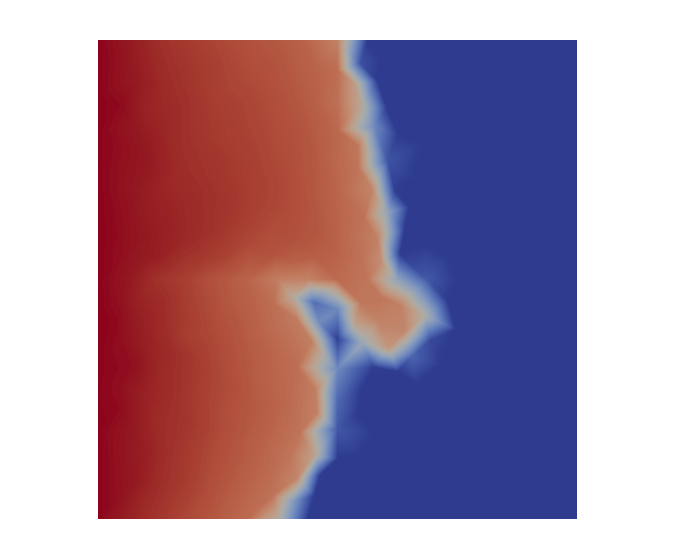
\includegraphics[width=.56\textwidth]{./Pics/HarmMeanCase/HarmMeanCase_Saturation_t_1dot15.png}
      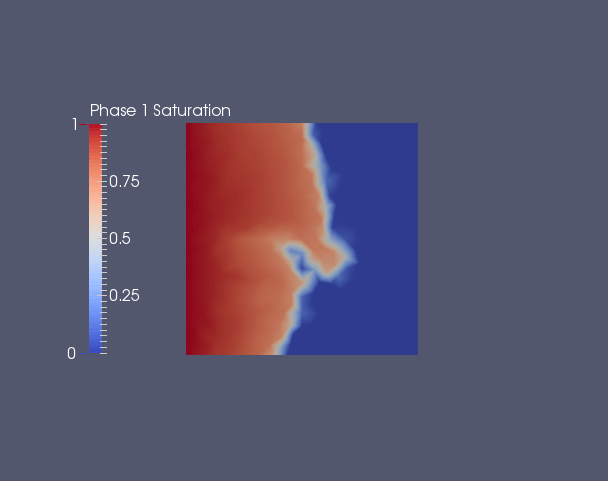
\includegraphics[width=.56\textwidth]{./Pics/PDFCase/PDFCase_Saturation_t_1dot15.png} 
      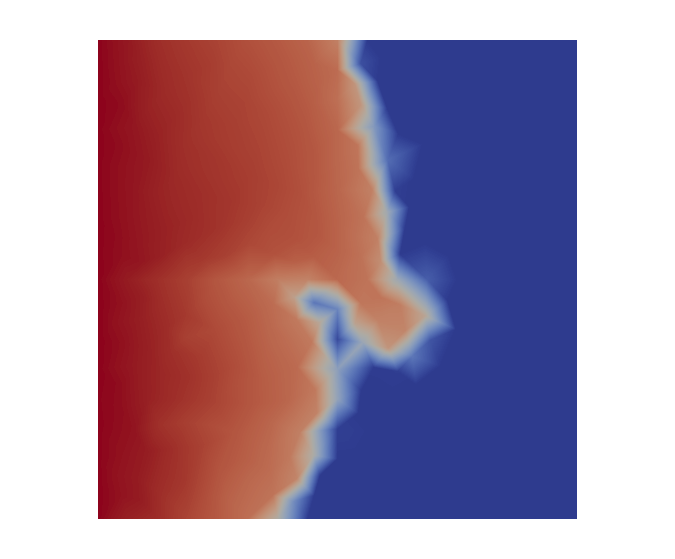
\includegraphics[width=.56\textwidth]{./Pics/SVDCase/SVDCase_Saturation_t_1dot15.png}}
\vspace{0.cm}
\hbox{ \hspace{0cm} (c) HarmMeanCase: Saturation (t=1.15s) \hspace{0.5cm} (d) PDFCase: Saturation (t=1.15s) \hspace{1.5cm} (e) SVDCase: Saturation (t=1.15s)}
\vspace{0.cm}
}   
\caption{Comparing the phase 1 saturation field for all the models at t=1.15s}
\label{fig:Saturationfield@t=1.15s}
\end{figure}
\end{landscape}
\clearpage
